
\section{Propuesta de solución}

	La solución propuesta consiste en una aplicación móvil en la plataforma Android, la cual nos ayudará a realizar la interpretación de voz a lenguaje de señas y la síntesis de voz a partir de un teclado.

	Se plantea la situación en la que una persona sorda, muda o sordomuda y una persona que puede escuchar y hablar perfectamente pero no conoce el lenguaje de señas están de frente y desean entablar una comunicación.

	La propuesta es tener una aplicación en el dispositivo móvil que ayude a estas dos personas a llevar a cabo una comunicación básica, con frases comunes. La aplicación contará con un módulo de reconocimiento de voz y bajo entrenamiento podrá reconocer ciertas frases de la comunicación como pueden ser frases para saludar, comprar o pedir indicaciones de la ciudad, y mediante la pantalla del móvil mostrar la imagen correspondiente en lenguaje de señas, de esta forma la persona 1 (persona que utiliza el lenguaje de señas) podrá entender lo que la persona 2 (persona que no utiliza el lenguaje de señas) quiere comunicar (Figura \ref{comunicacionVoz}).

	\begin{figure}[H]
		\centering
		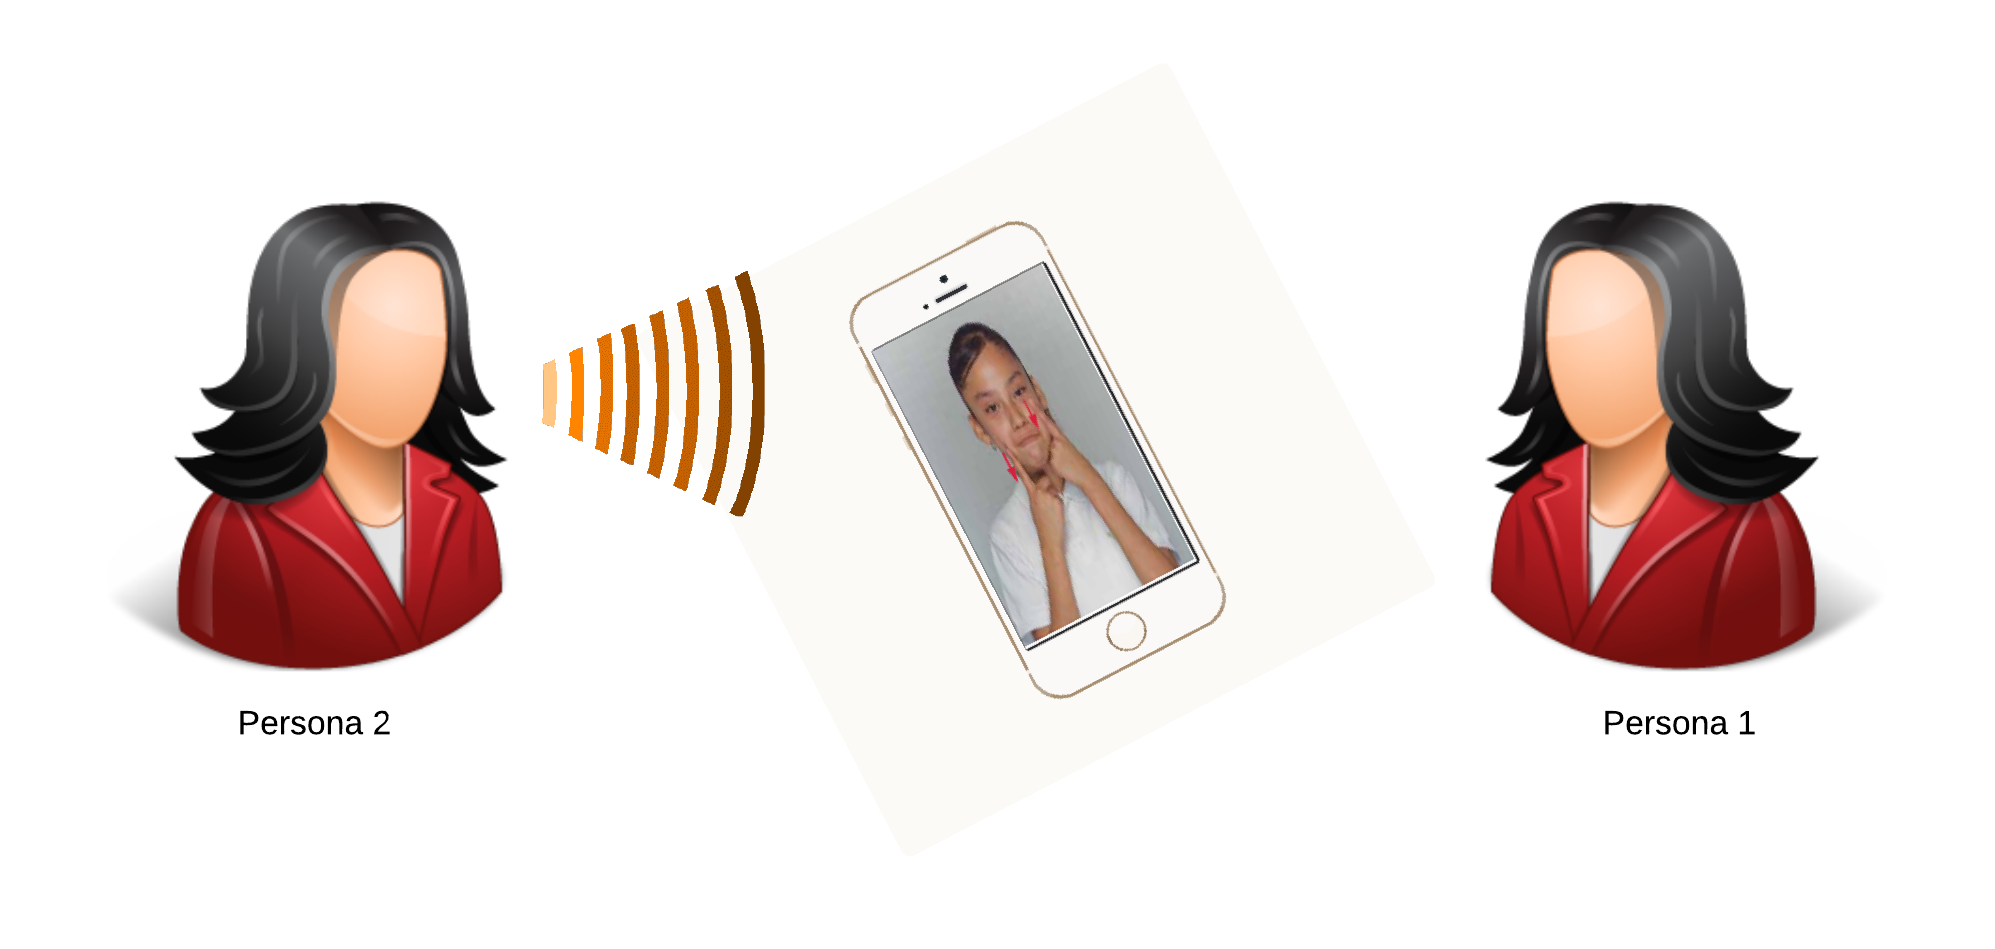
\includegraphics[scale = 0.7]{figures/ComunicacionBA}
		\caption{Comunicación por voz.}
		\label{comunicacionVoz}
	\end{figure}

	Por otra parte, cuando la persona 1 quiera comunicarse con la persona 2, la aplicación en esta sección mostrará un teclado por el cual la persona 1 escribirá la frase que desea comunicar y se sintetizará en voz lo escrito, el módulo se plantea de tal forma que se pueda obtener la comunicación bidireccional y ésta no quede trunca (Figura \ref{comunicacionTeclado}), la implementación de esta sección se hará con el uso de la API de síntesis de voz de Google, de tal manera que el trabajo esté enfocado principalmente en la primera sección que es el reconocimiento de voz. Esto se propone para que la app final permita una comunicación bidireccional.

	\begin{figure}[H]
		\centering
		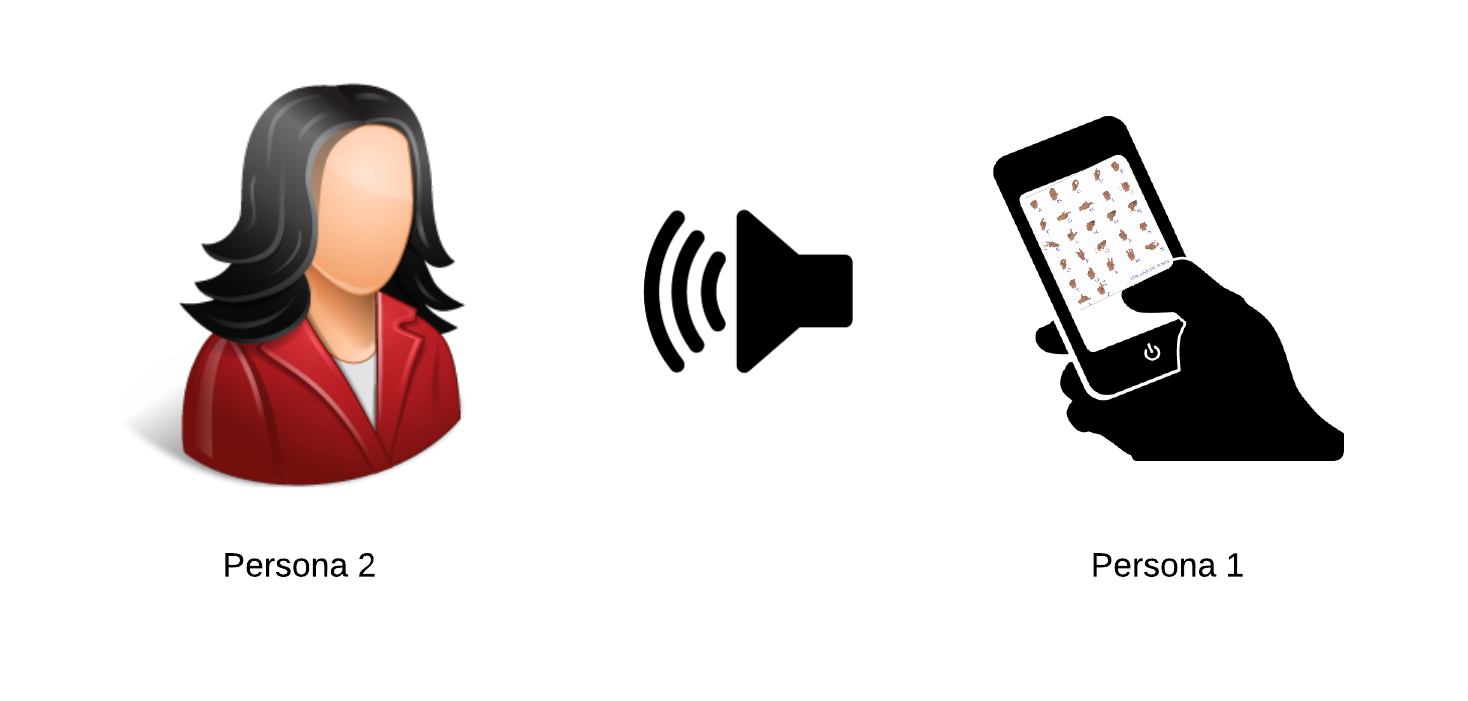
\includegraphics[scale = 0.8]{figures/ComunicacionAB}
		\caption{Comunicación por teclado}
		\label{comunicacionTeclado}
	\end{figure}
	
	Además de los módulos propuestos se plantea que la aplicación cuente con un diccionario, con el cual podremos aprender el lenguaje de señas, palabras, gestos y el cómo utilizarlos.

		\subsection*{Arquitectura del sistema.}
		
		Se puede definir a la aplicación en diferentes módulos, los cuales se pueden observar en las Figuras \ref{vozSenB} y \ref{tecVozB}.
		En la Figura \ref{vozSenB} se explicará cómo sería la arquitectura de la parte de la aplicación donde se va a tener la comunicación por voz.

		\begin{figure}[H]
			\centering
			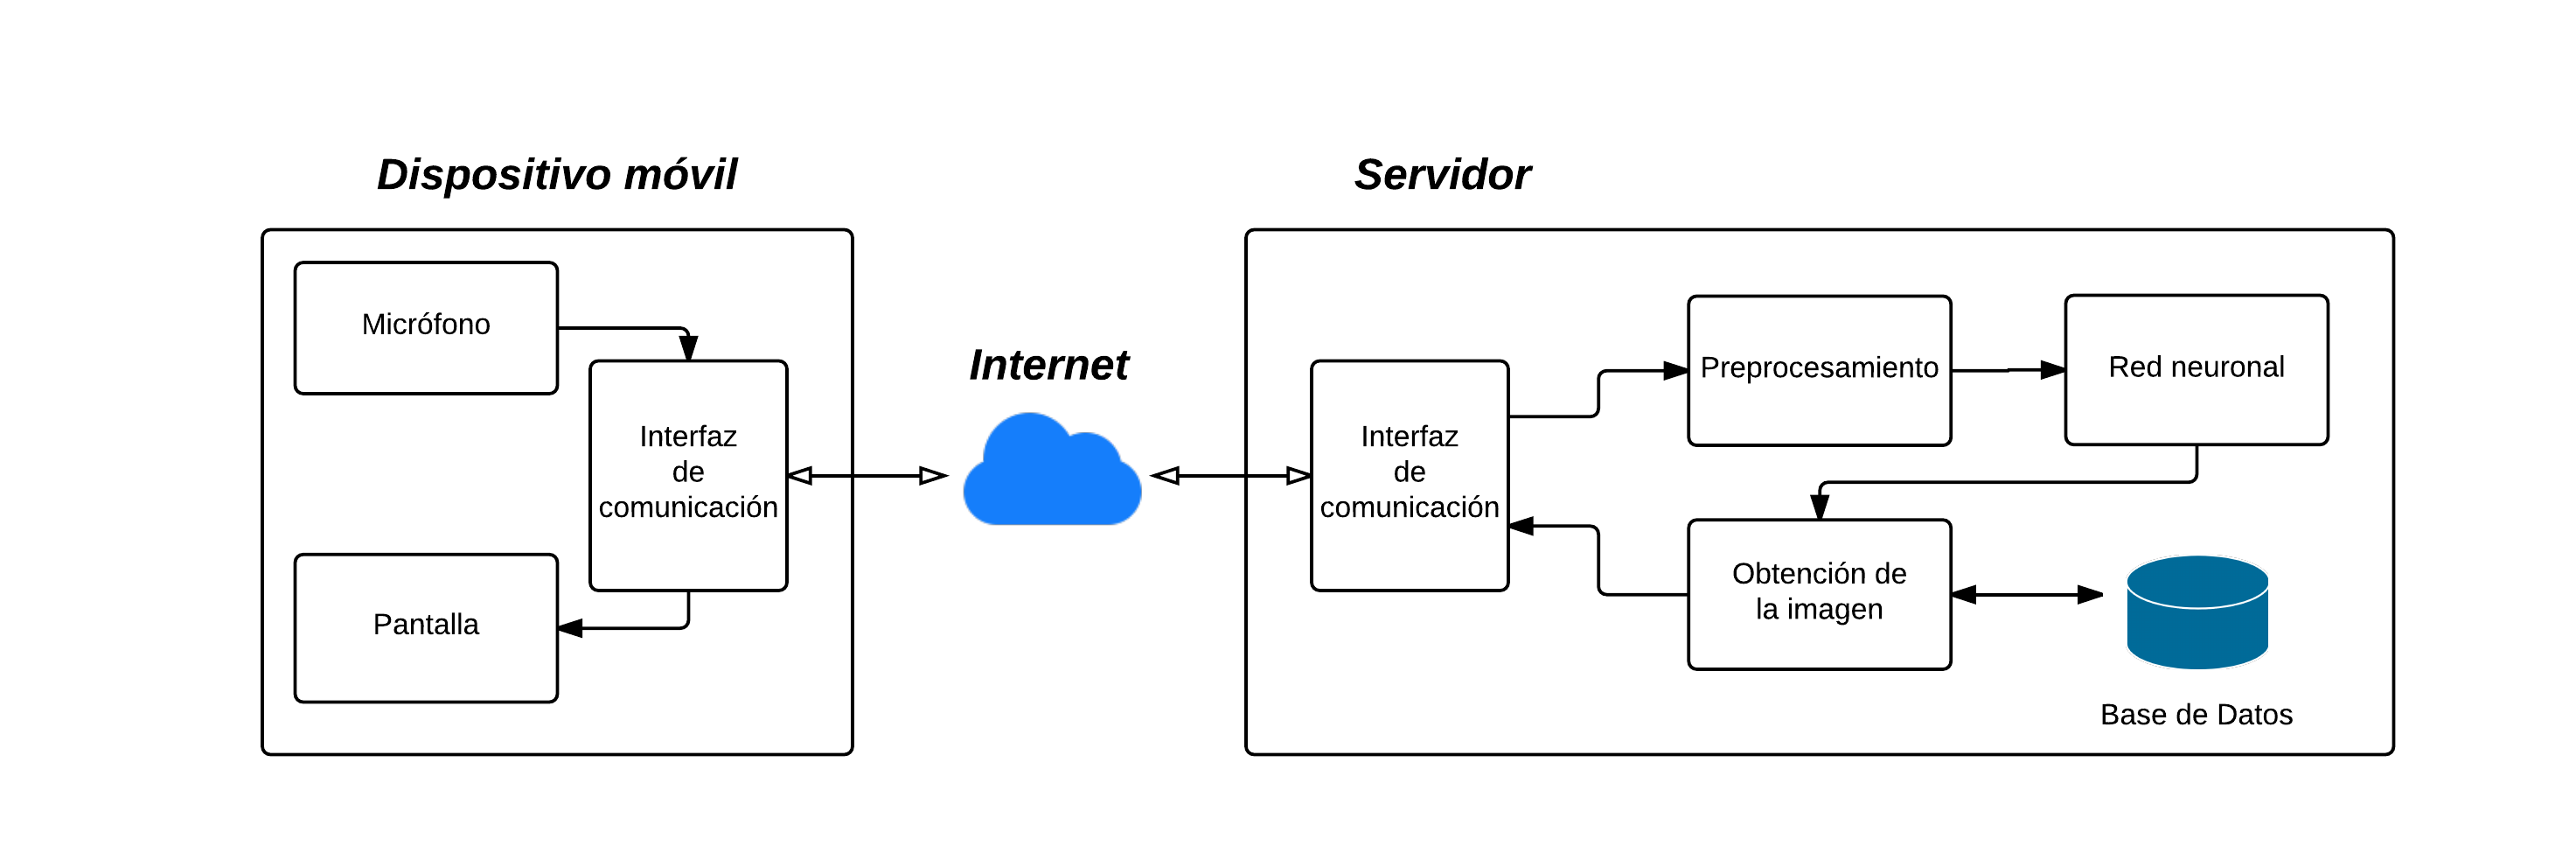
\includegraphics[scale = 0.7]{figures/Etapavoz}
			\caption{Diagrama a bloques del sistema que relaciona voz a imágenes de lenguaje de señas.}
			\label{vozSenB}
		\end{figure}		

		A través del micrófono del dispositivo móvil se va a capturar la señal de voz, esta señal será enviada a través de internet a un servidor que realizará el pre procesamiento de ésta para su posterior reconocimiento y obtención de la imagen correspondiente a la frase identificada, finalmente la imagen recuperada será enviada al móvil para su presentación en la pantalla.
		\paragraph{}

		En la Figura \ref{tecVozB} se presenta la arquitectura del módulo de síntesis de voz donde la entrada del texto es por medio del teclado.

		\begin{figure}[H]
			\centering
			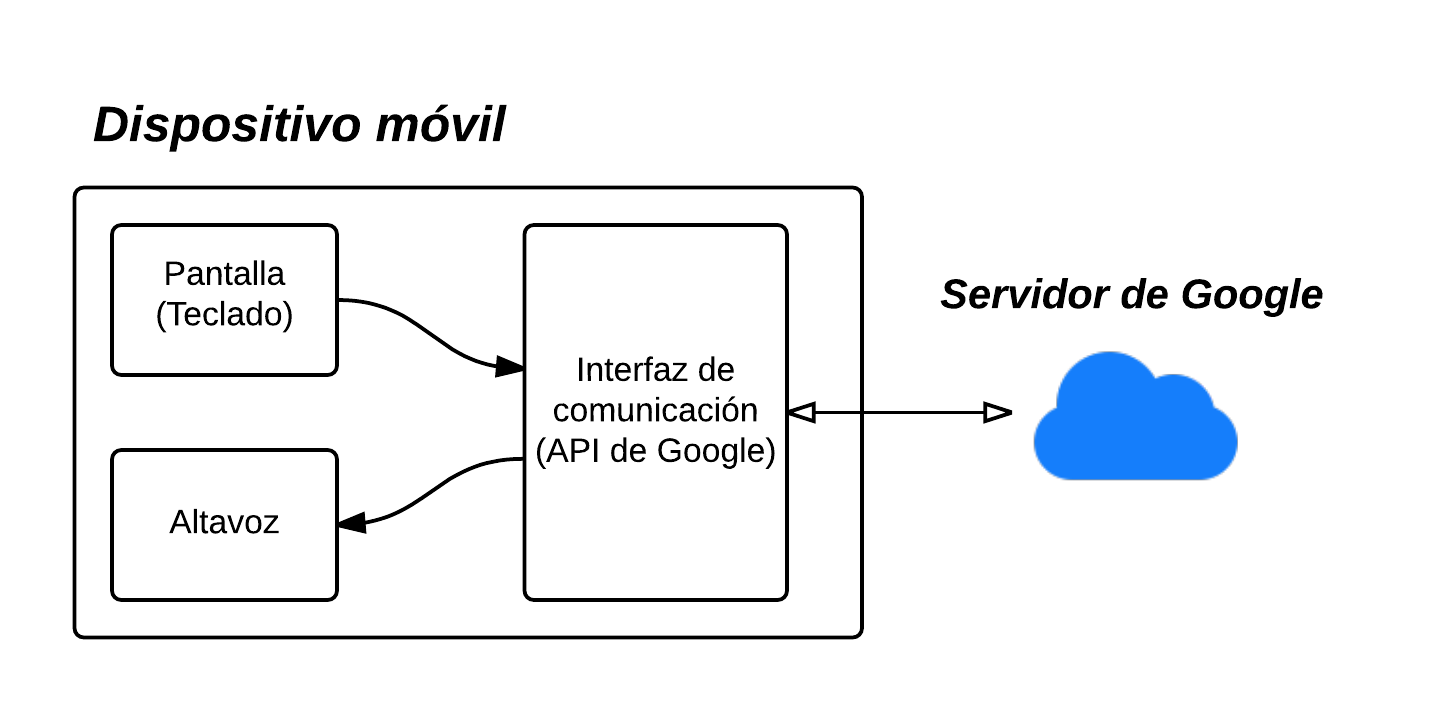
\includegraphics[scale = 0.8]{figures/Etapateclado}
			\caption{Diagrama a bloques del módulo de síntesis de voz con entrada por medio de un teclado.}
			\label{tecVozB}
		\end{figure}	

		Por medio de un teclado presentado en pantalla se tendrá la entrada del texto que se desea comunicar y con ayuda de la API de síntesis de voz de Google  se implementará la síntesis para que la persona 2 escuche lo que la persona 1 quiere comunicar.





	\subsection*{Metodología}
	
	Para implementar la aplicación propuesta se plantea realizar las siguientes actividades.

	\begin{itemize}
		\item Reconocimiento de voz: Como parte del pre procesamiento se hará un análisis de las características de la voz que debemos tratar para realizar dicho reconocimiento, de este análisis implementaremos determinados filtros que nos ayuden a preparar la señal de voz para el adecuado procesamiento. Se estudiarán las redes neuronales adecuadas para llevar a cabo el reconocimiento de frases. El entrenamiento y validación de la red primeramente se llevará a cabo en Matlab debido a su fácil manejo y después se implementará en el lenguaje de programación C debido a que el desempeño será mejor que la implementación en Java.

		Se opta por el uso de redes neuronales para el reconocimiento de voz debido a que se tiene más experiencia en el tema y de esta forma permitir realizar la aplicación completa dados los tiempos para el desarrollo del proyecto.

		\item Base de datos: Se implementará una base de datos relacional en MySQL que almacenará todo el vocabulario seleccionado del lenguaje de señas relacionado a su texto correspondiente, de esta forma cuando se tenga la frase se pueda solicitar la imagen.

		Se decidió usar MySQL por ser el manejador de bases de datos más versátil de los tres más comerciales\footnote{MySQL, SQL Server y PostgreSQL}, esta decisión se toma con base a los datos mostrados en la tabla \ref{tabla:dbms}.

		\item Síntesis de voz: Se llevará a cabo la implementación de la síntesis de voz de las  frases ingresadas a través del teclado con ayuda de la API de Google, se estudiará el funcionamiento de la API y se analizará la mejor implementación posible que pueda usarse, ya sea mediante una conexión a internet o de forma local.

		\item Aplicación móvil: Se realizará el diseño de la aplicación de tal forma que sea intuitiva, se definirá el modelo de desarrollo que mejor se adapte a la aplicación y se especificarán los requerimientos del sistema.

		\item Conectividad: Se implementará la comunicación entre el servidor y el dispositivo móvil por medio del protocolo TCP-IP para tener acceso a la red y de esta forma poder manipular la base de datos a nuestra conveniencia, de esta forma, la aplicación necesitará la conexión a internet para llevar a cabo el procesamiento, la conexión puede ser tanto por Wi-Fi como por redes móviles.

		\item Integración y validación: Ya teniendo todos los elementos del sistema se llevará a cabo la integración y validación del sistema, básicamente enlazar los puntos principales en el servidor y realizar la conexión con el dispositivo móvil a través de la internet.

		\item Pruebas: Finalmente se llevarán a cabo diversas pruebas en diferentes escenarios en los que se requiera la comunicación entre personas que presentan la deficiencia para hablar y las personas que no la presentan.

		\item Para cuestiones técnicas se hará un análisis de la velocidad de respuesta del sistema de forma teórica, esto tomando la complejidad computacional y la velocidad de procesamiento donde se llevará a cabo el reconocimiento.
	\end{itemize}